\documentclass[12pt,a4paper]{article}

\usepackage{epcc}
%\usepackage{graphics}
\usepackage{graphicx}
\usepackage{pgfgantt}
\usepackage{array}

% This example file shows how a thesis can be laid out using Latex. It
% does not use any special local features so should be portable to other
% places.
%
% To produce myfile.pdf from myfile.tex type:
% 
% pdflatex myfile
%
% Note that pdflatex expects all included figures to be in PDF too. See
% the includegraphics command below.


% This document contains many cross-references and forward references,
% eg in constructing a table of contents, so Latex may need to be run
% twice to get all the references correct. If you need to run Latex twice
% you may get the warning:
% 
% LaTeX Warning: Label(s) may have changed. Rerun to get cross-references right


\begin{document}

\title{Software Development\\Planning and Risks}
\author{B098688 - s1671778}
\date{\today}

\makeEPCCtitle

\thispagestyle{empty}

\newpage

\pagenumbering{roman}

\tableofcontents


\newpage
\pagenumbering{arabic}

\section{Introduction}

This report will provide a series of guidelines on how to proceed with the creation of a web application. The web application's code has been initiated by an unknown party, that is written in \texttt{html}, \texttt{JavaScript}, \texttt{python} and uses the web framework \texttt{flask}. Said code must be enhanced such that it fulfills the base requirements for the project. The skeleton of the web application has a few elements already built in. It is, however, very rough and needs much work to become a feasible end product. 

The first part of the report will briefly outline what is the intended project, and the background needed to understand what it is attempting to achieve. While this is being discussed, some of the important factors to keep in mind are highlighted. After this is done, several comments regarding issues in the provided code are made. Afterwards, solutions for most of these are proposed, and eventually presented in a \textit{time/effort} estimation plan. Finally, once the project has been understood, and its purpose is clear, risk analysis and management strategy are posed. For the latter, a Gantt chart is put together to act as a guide for the next steps: \textit{UI and Evaluation Plan} and \textit{Refactoring and Reflection}.

The management strategy in this small project will help make a successful end product. There are many factors to be analysed in order to properly develop the software development planning. Considering personal inexperience in web security, \texttt{flask}, \texttt{html}, and \texttt{JavaScript}, it is safe to assume that many issues with the program will be overlooked at the beginning. This means that the problems mentioned in this document will be a fraction of those that will actually be fixed in the later stages of the project. This will require allocating time to research on the aforementioned topics as well as choosing carefully the best development model. After careful consideration and taking into account that this project will need to cycle from the current code to an improved version a few times, the \textit{Waterfall with Subprojects} development model is going to be used.

Having mentioned how the lack of experience will impact the development model required, it is important to analyze how it will modify other elements of the project's progress. The best way to do this is most likely through the Gantt chart. In it, tasks that have to be completed and are related to areas of inexperience will need some time allocation for 'research' or 'practice', but this will decrease as more tasks of the same area are performed, i.e. account for knowledge growth. 

\section{Project Specifications}

The goal is to further develop a web based application that allows the user to generate a squad (Warband) for a tabletop game - with certain constraints. The application must allow users to create and edit squads with an unchangeable name, no more than 10 members, and no fewer than 1. The user begins with a Captain, that can become better with time, and has a limited amount of money to hire other regular team members, that cannot improve with time, and a special member, the Ensign, who, like the Captain, can evolve in time.

The idea of the web application is to check that all constraints are fulfilled for a user's Warband, and that if one or more are violated, a warning message is displayed such that the user is able to modify their decision. The base stats for each team member are shown in the Annex.

\subsection{New Warband}

A new Warband begins with \textbf{one} Captain and \textbf{500} credits. For a new Warband to be created, the following conditions must be met:

\begin{enumerate}
 \item Warband Name.
 \item Player Name.
 \item Positive number of credits.
 \item Captain: \begin{enumerate}
                 \item \textbf{ONE} per Warband.
                 \item Starts with \textbf{one} EXPERIENCE.
                 \item Must be assigned \textbf{one} SPECIALISM (Engineering, Psychology, Marksman, Tactics, Melee, Defence).
                 \item \textbf{One} Associated Skill must be assigned to the specified SPECIALISM: \begin{enumerate}
							  \item Engineering: [Repair, Sabotage, Augment].
							  \item Psychology: [Bolster, Terror, Counter].
							  \item Marksman: [Aim, Pierce, Reload].
							  \item Tactics: [Squad, Ambush, Surround].
							  \item Melee: [Block, Riposte, Dual].
							  \item Defence: [Shield, Sacrifice, Resolute].
							 \end{enumerate}
				 \item Must be given \textbf{one} WEAPONS/EQUIPMENT: \begin{enumerate}
				                                         \item Blaster: \textbf{5} credits.
				                                         \item Needle Gun: \textbf{12} credits.
				                                         \item Blade: \textbf{3} credits.
				                                         \item Cannon: \textbf{15} credits.
				                                         \item Whip: \textbf{5} credits.
				                                        \end{enumerate}
                \end{enumerate}
 \item Ensign: \begin{enumerate}
                \item Price of hiring: \textbf{250} credits.
                \item Maximum \textbf{ONE} (Warbands can be created without an Ensign).
                \item Must be assigned \textbf{one} SPECIALISM.
                \item Must be assigned \textbf{one} Associated Skill.
                \item Must be given \textbf{one} WEAPONS/EQUIPMENT.
               \end{enumerate}
 \item The total number of members is \textbf{10} (including the Captain and Ensign).
 \item Prices of hiring are: \begin{enumerate}
                              \item Augment Gorilla: \textbf{20} credits.
                              \item Lackey: \textbf{20} credits.
                              \item Security: \textbf{80} credits.
                              \item Engineer: \textbf{60} credits.
                              \item Medic: \textbf{50} credits.
                              \item Commando: \textbf{100} credits.
                              \item Combat Droid: \textbf{150} credits.
                             \end{enumerate}
\end{enumerate}

\subsection{Edit Warband}

When editing a Warband there is also a set of conditions that have to be met. They are outlined here.

\begin{enumerate}
 \item Can hire squad members as long as the total number of squad members does not exceed \textbf{10}, and as long as the Warband's number of credits does not become negative.
 \item Captain and Ensign can gain EXPERIENCE.
 \item Acquired EXPERIENCE can be traded for upgrades for Captain and Ensign (\textbf{10} EXPERIENCE points can be turned into \textbf{1} point for a Stat up to specified maximum values shown in the Appendix section).
 \item Can remove squad members, but their hiring price is \textbf{not} returned to the number of credits.
 \item The Captain can have up to \textbf{two} weapons and \textbf{four} items.
 \item The Ensign can have up to \textbf{one} weapon and \textbf{3} items.
 \item Weapons cost credits. Changing or adding weapons \textbf{cannot} result in a negative number of credits.
\end{enumerate}


\section{Identified Problems}

Now that the constraints of the teams have been covered, it is possible to go through the code to check missing or wrong information. But first, going through the current web application to see errors in its functioning is important. The following is a list of problems that are observed by working though the web application alone. 

\subsection{New Warband}

\begin{enumerate}
 \item The most obvious deficiency is the fact that Warbands are not linked to a specific player. This means that anyone can edit any Warband. The game must support more than one player, where only the team's owner can edit it, but all other players can see it.
 \item There is no way to go from the ``New Warband'' or ``Edit Warband'' pages to the ``Home'' page without using browser back button or address bar.
 \item There has been no attempt at testing the current product. For example, when attempting to generate an illegal ``New Warband'' (Captain without weapon / skill / specialism), an error message is given, but no explanation or way to return and fix the mistakes are provided.\\
 \begin{minipage}[t]{\linewidth}
 \centering
 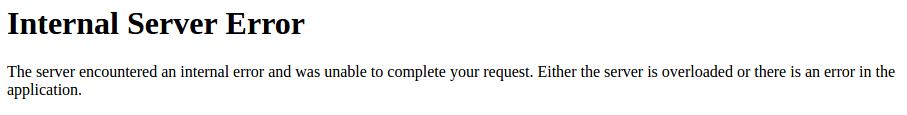
\includegraphics[width=1\textwidth]{img/warband_error}
 Generic error message.
 \end{minipage}
 
 \item The price of weapons is not discounted from the number of credits from the screen when creating a ``New Warband''.
 \item Neither Captain nor Ensign have ''Notes`` section, and merged ''Weapons and Equipment``, whereas the two should be different.
 \item The Ensign is called ``Apprentice'' for some reason - this is confusing.
 \item The cost of the ``Apprentice'' is 200 credits instead of 250 as it should. This and the previous item are actually related, and comprise a larger problem - the information from each team member is actually stored in the \texttt{python} code and separately in the \texttt{html/JavaScript} code. Due to this, the price on screen is 200 credits, but it actually subtracts 250 credits (as it should). 
 \item A 10 row table allows the player to fill out the form with up to 12 members (returns the generic error message when done so).\\
 \begin{minipage}[t]{\linewidth}
 \centering
 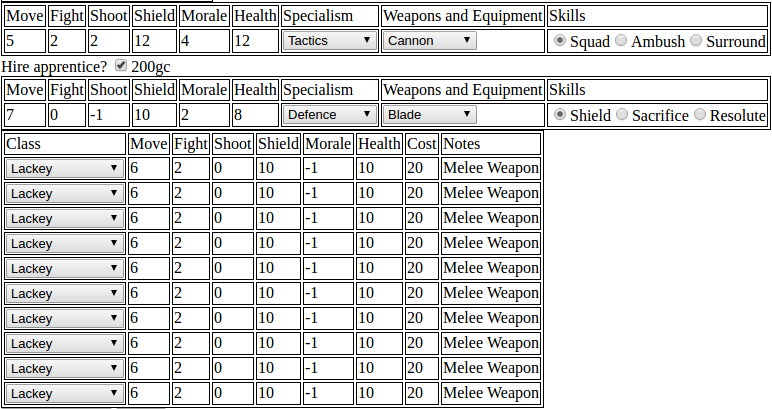
\includegraphics[width=1\textwidth]{img/twelve_members}
 Chance to include 12 members.
 \end{minipage}
 
 \item There is no method for handling attempts at creating a new Warband with a name that already exists. This has to be carefully thought out when including multiplayer - no two teams can have the same name, even if they are built by different players - involving the client is important for this decision.

\end{enumerate}

\subsection{Edit Warband}

\begin{enumerate}
 \item The most serious problem in the ``Edit Warband'' menu is the handling of credits. When editing the Warband the number of credits is modified erroneously:\\
 A new Warband with only a Captain with a cannon (15 credits) is generated. Then, in the ``Edit Warband'' page, clicking ``Create Warband'' decreases the number of credits by 15 (shown in the figures below). Like this, there are other errors with the credit handling in the ``Edit Warband'' page.\\
 \begin{minipage}[t]{\linewidth}
 \centering
 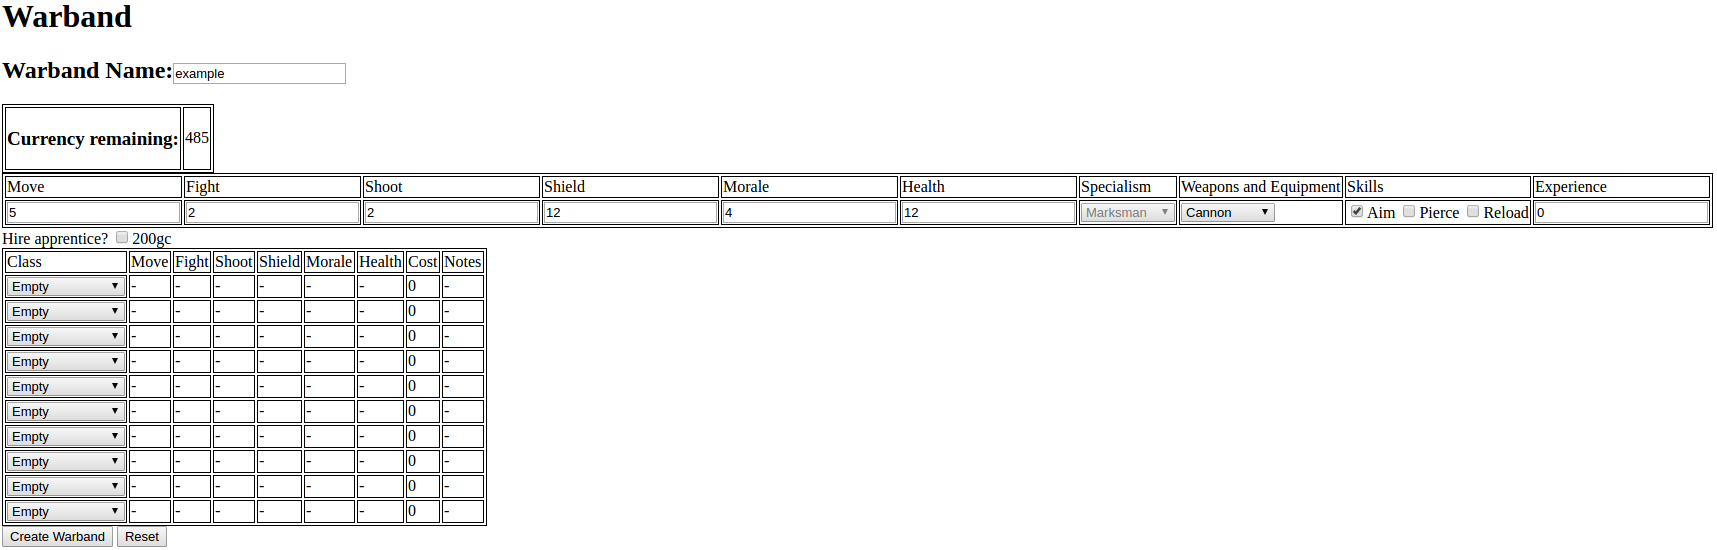
\includegraphics[width=1\textwidth]{img/example0}
 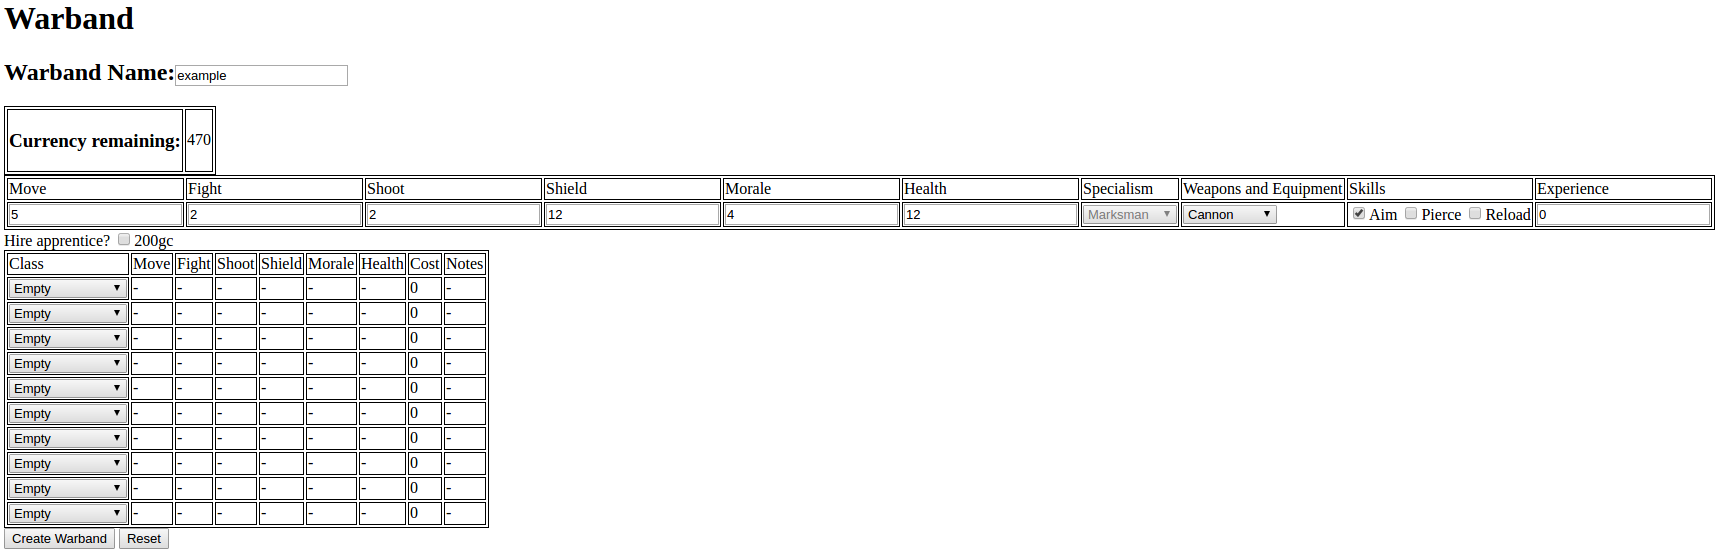
\includegraphics[width=1\textwidth]{img/example1}
 \end{minipage}
 
 \item It is not possible to hire an Ensign after creating the Warband.
 \item Squad members are treated like slaves, i.e. it is possible to sell them for the original amount of credits that they were ``hired'' with. This needs to change according to the game rules.
 \item The rules for increasing the Captain's and Ensign's skills is completely off - it is unlimited and completely uncorrelated to the experience points. 
 \item The Captain and Ensign maximum values of skills (Annex) are not taken into consideration.
 \item Captain is not able to have \textbf{two} weapons.
 \item Neither Captain nor Ensign can obtain equipment.
 \item When attempting to make an illegal Warband nothing happens - not even the generic error message returned previously.
 \item Impossible to add number of credits.
\end{enumerate}



\section{Project Planning}

\newganttchartelement{voidbar}{
    voidbar/.style={
        draw=black,
        top color=black!25,
        bottom color=black!23
    }}
    \begin{ganttchart}[x unit=0.42cm, 
        y unit title=0.7cm,
        y unit chart=0.5cm, vgrid, title label font=\footnotesize,
        canvas/.style={draw=black, dotted}]{1}{28}
        \gantttitle{Hours}{28}\\
        \gantttitlelist{0,5,10,15,20,25,30,35,40,45,50,55,60,65}{2} \\

        \ganttbar{A}{1}{2}     \\ 
        \ganttbar{B}{3}{6}    \\   
        \ganttbar{C}{7}{8}              \\ 
        \ganttbar{D}{9}{12} \\
        \ganttbar{E}{13}{16} \\
        \ganttbar{F}{17}{20} \\
        \ganttbar{G}{7}{8} \\
        \ganttbar{H}{9}{12} \\
        \ganttbar{I}{13}{16} \\
        \ganttbar{J}{16}{21} \\
        \ganttbar{K}{7}{7} \\
        \ganttbar{L}{8}{11} \\
        \ganttbar{M}{12}{14} \\
        \ganttbar{N}{15}{16} \\
        \ganttbar{O}{17}{20} \\
        \ganttbar{P}{21}{24} \\
        \ganttbar{Q}{25}{28} \\
        \ganttbar{R}{28}{28} \\
    \end{ganttchart}

One of the important restrictions of the model is that neither hares nor 
pumas can live in sections that represent water. Therefore it is 
straightforward to expect 
that if a landscape is entirely covered in water it should run faster than one 
completely covered 
in land, since no computations related to the population densities should be 
required. This is the motivation behind the first performance test.

For an input file of fixed size the percentage of land to water is varied from 
$0\%$ to $100\%$. Using a bash script, the time it takes to run the program 
with different l


The output confirms the intuition that the program's run time should increase 
as the percentage of land in the input landscape file is increased. 
Furthermore, it shows that the aforementioned growth has a direct 




\section{Code Profiling}

In order to actually know which functions make up for most of the time in the 
run time for the program, the python native profiler ``\texttt{cProfile}'' was 
used. First, two input files of the same size ($100$x$100$) one with $30\%$ and 
the other $60\%$ land-to-water ratios were profiled. The output shows how much 
time each function took and how many times they were called. These results are 

These figures provide a more complete picture of what can be done to optimize 
the program under study. The first thing that is evident is that 
\texttt{ppm.py} is using most of the run time in all four cases. This file 
holds the functions that are used to generate the \texttt{.ppm} files. Hence 
this is where it would be most beneficial to attempt some type of 
optimization. Additionally, the second set of pie charts makes it clear that 
the files \texttt{population.py} and \texttt{landscape.py} are also good 
candidates for possible optimization.


\section{Conclusions}

After performing a series of performance and profiling tests on the program 
written by \textit{Callum Black, Andr\'es Cathey, and Eskil Joergenssen} for the 
HPC course \textbf{Programming Skills} a few good features can be made 
about the 
run times of said program. Additionally, it was possible to know what functions 
should be optimized in order to do a significant impact on the program's run 
time.

The first feature of the code that was studied was how the program's run time 
increases as the land-to-water percentage is increased. A linear relation 
between these was found, confirming that the computation time increases when 
the percentage of land in a fixed size file is increased. 

Afterwards, it was shown that the program's run time also grows linearly when 
the input landscape file's number of land/water squares is increased linearly. 
This confirmed the intuition that the most important factor for the program's 
run time is the landscape's area. 

Finally, the profiling part of the tests provided information as to what 
functions could be optimized in order to decrease the run-time of the program. 
Said optimizations should be done for writing the \texttt{.ppm} file, since 
this always represents most of the run time regardless of input file size (the 
percentage of the run time that it represents should also grow linearly).

It can be concluded that performance testing and profiling are important to 
know what are the weaknesses and the strengths of large, or complex, codes that 
cannot be studied by simply going through them. These methods are also very 
useful to know what sections of a code is taking up most of the run time and, 
thus, best suited for optimization.

\newpage

\section{Annex}

\subsection{Base stats}

Besides the stats shown in table~\ref{Atable:1}, both Captain and Ensign start with empty Skillset (that has to be filled when creating a squad), as well as an Associated Specialism, and no Items (one Weapon has to be added when creating a squad). All other stats are summarized in the following table.

\begin{table}[h]
\begin{center}
\begin{tabular}{|m{1.8cm}|c|c|c|c|c|c|c| m{2.1cm} |}
\hline
{\bf Squad Member} & {\bf Move} & {\bf Fight} & {\bf Shoot} & {\bf Shield} & {\bf Morale} & {\bf Health} & {\bf Cost} & {\bf Experience}\\
\hline
  Captain & 5 & 2 & 2 & 12 & 4 & 12 & 0 & 0\\
  \hline
  Ensign & 7 & 0 & -1 & 10 & 2 & 8 & 250 & 0\\
  \hline
  & & & & & & & & {\bf Notes} \\
  \hline
  Augment Gorilla & 8 & 3 & 0 & 10 & 2 & 8 & 20 & Animal, cannot carry treasure or items\\
  \hline
  Lackey & 6 & 2 & 0 & 10 & -1 & 10 & 20 & Melee Weapon\\
  \hline
  Security & 6 & 2 & 1 & 12 & 2 & 12 & 80 & Blaster, Blade\\
  \hline
  Engineer & 4 & 0 & 3 & 12 & 2 & 10 & 60 & Blaster, Repair Kit\\
  \hline
  Medic & 5 & 0 & 0 & 12 & 3 & 10 & 50 & Blade, Medkit\\
  \hline
  Commando & 8 & 4 & 0 & 10 & 4 & 12 & 100 & Stealth Suit, Blade, Needle Gun\\
  \hline
  Combat Droid & 3 & 2 & 4 & 14 & 0 & 14 & 150 & Mechanoid, Dual Blaster, Claws\\
\hline
\end{tabular}
\end{center}
\caption{Base stats for each squad member.}
\label{Atable:1}
\end{table}

\newpage

\subsection{Maximum Stats}

As the Captain and Ensign are able to increase their stats, it's important to state their maximum stats. In order to increase any of these stats by \textbf{1} point, the corresponding squad member (Captain or Ensign) will loose \textbf{10} EXPERIENCE points. In one edit no stat can be increased by \textbf{more than 1} point.

\begin{table}[!ht]
\begin{center}
\begin{tabular}{|c|c|c|c|c|c|c|c|}
\hline
{\bf Squad Member} & {\bf Move} & {\bf Fight} & {\bf Shoot} & {\bf Shield} & {\bf Morale} & {\bf Health}\\
\hline
  Captain & 5 (+0) & 2 (+8) & 2 (+8) & 12 (+0) & 4 (+8) & 12 (+8)\\
  \hline
  Ensign & 7 (+0) & 0 (+6) & -1 (+6) & 10 (+0) & 2 (+4) & 8 (+8)\\
\hline
\end{tabular}
\end{center}
\caption{Maximum stats for Captain and Ensign.}
\label{simple_table}
\end{table}



%\begin{thebibliography}{100}

%\bibitem{ref:lam} L.Lamport. {\em 1986 Latex User's Guide
%and Reference Manual.} Addison Wesley. pp242.

%\bibitem{ref:bloggs} F.Bloggs. {\em 1993 Latex Users do it
%in Environments} Int. Journal of Silly Findings. pp 23-29.

%\end{thebibliography}


\end{document}

